\chapter{Asking Supercar Owners How They Got Rich!}

This lecture is not a blackboard derivation in the usual sense, but it does unfold a definite mechanism. We begin with the visible trophies of wealth---cars, houses, revenue claims, exits---and then we ask what machine lies behind them. As the interviews accumulate, a repeated structure emerges: one first creates active income, one then decides whether to burn that income on lifestyle or convert it into an asset base, and only after that conversion does durable cash flow appear. The chapter follows that order closely, because the lecture itself teaches by staging the puzzle first and only later disclosing the bookkeeping.

\section{Opening Montage and the Miami Question}

The lecture opens with a rapid montage of claims. One man says he works in construction and real estate; another says he sold a business for \$115 million; another says a \$20 million home is serviced by passive income; another says his company did roughly \$35 million in a year and is valued at about \$140 million; another insists that without sales there is no money; still another would rather have a billion followers than a billion dollars. The host does not yet explain any of this. He piles the claims up and lets the tension sit.

Then comes the framing question. Miami is presented as a city overflowing with supercars, and so the lecture asks what these people actually do and, more importantly, what financial structures support what we see. We should take that seriously. The car is not the object of analysis. The car is a boundary condition. The real object is the vehicle beneath the vehicle.

\begin{definition}
In this chapter, a \emph{vehicle} is any structure that converts present effort or capital into future cash flow or future sale value. The lecture offers several such vehicles: operating businesses, real estate, audience and distribution, and, in one speaker's account, policy-based compounding with collateralized borrowing.
\end{definition}

The montage therefore does two things at once. It promises spectacle, and it quietly establishes the variables that will return throughout the lecture:
\begin{itemize}
\item current income,
\item revenue,
\item enterprise value,
\item asset cash flow,
\item and the question of whether consumption comes first or last.
\end{itemize}

\section{Eric Spofford: From Personal Collapse to a Wealth Machine}

The first full case is Eric Spofford, and the lecture is careful with the order. We do not begin with his money. We begin with his life. He says he came out of crime, addiction, and street life; he says he got sober at age twenty-one in 2006; he says he entered drug-addiction treatment and then built a business that helped other people get sober. Only after that biographical sequence is in place does the host ask about the largest year of money.

That question elicits the first large numerical ledger of the lecture. Eric says the biggest year was a little more than \$100 million. He says he built the business from the ground up and sold it for \$115 million. He also says that he sold underlying real-estate assets for roughly \$40 million. The point here is not merely that the numbers are large. The point is that the lecture ties those numbers to a specific chain: work, business construction, real-estate development, exit.

We may record the stated amounts as follows:
\begin{align}
\text{Business sale} &\approx \$115\,\text{M},\\
\text{Underlying real-estate sales} &\approx \$40\,\text{M}.
\end{align}

Eric then makes the decisive turn. He says that real estate is now a main focus of his, and when he talks about luxury consumption he does not describe it as a direct output of a paycheck. He says, rather, that the G-Wagon, the Cullinan, and the mortgage on the \$20 million home are paid for by passive income and free cash flow. That is the central sentence of the lecture. The luxury object is downstream. The asset machine is upstream.

A schematic transcription of that mechanism is
\begin{equation}
A \longrightarrow Y_{\mathrm{passive}},
\end{equation}
where \(A\) denotes an asset base and \(Y_{\mathrm{passive}}\) the recurring cash flow that the asset base throws off.

At this point the lecture has moved from biography to mechanism. We are ready for the real conceptual obstacle.

\subsection{Question \& Answer}

\paragraph{Question.} Why do people who make a great deal of money so often fail to become wealthy in a durable way?

\paragraph{Answer.} Because making income and preserving wealth are not the same operation. The lecture's answer is that many people stop at the first stage. They create active income and then immediately convert it into lifestyle. The wealthier path is different: one takes the surplus generated by active income and turns it into assets that keep paying after the first burst of effort is over.

We can formalize the bookkeeping this way. Let \(W_t\) be wealth at time \(t\), let \(Y_{\mathrm{active}}(t)\) be active income, let \(Y_{\mathrm{passive}}(t)\) be cash flow from assets, and let \(C_t\) be consumption. Then
\begin{equation}
\Delta W_t = Y_{\mathrm{active}}(t) + Y_{\mathrm{passive}}(t) - C_t.
\end{equation}

If there is active income but no asset machine, then the lecture's warning is that the surplus vanishes into lifestyle. We may write
\begin{equation}
S_t = Y_{\mathrm{active}}(t) - C_t,\qquad A_{t+1}=A_t+S_t.
\end{equation}
If \(S_t\) is small because consumption rushes upward with income, then the asset base does not thicken. If \(S_t\) is directed into assets, then a second flow appears.

Eric himself phrases the contrast with a memorable image: a pile of money versus a river of money. This can be translated into two update rules.

For a mere pile,
\begin{equation}
W_{t+1}^{\mathrm{pile}} = W_t^{\mathrm{pile}} - C_t.
\end{equation}
For a river-producing asset base,
\begin{equation}
W_{t+1}^{\mathrm{river}} = W_t^{\mathrm{river}} + Y_{\mathrm{passive}}(t) - C_t.
\end{equation}

The point becomes clearer if we unfold this for several periods.

\begin{enumerate}
\item Suppose first that one has only a stock of money.
\item After \(n\) periods of spending, one has
\begin{equation}
W_n^{\mathrm{pile}} = W_0 - \sum_{t=0}^{n-1} C_t.
\end{equation}
\item Now suppose instead that one has built an asset base producing recurring inflow.
\item Then after \(n\) periods one has
\begin{equation}
W_n^{\mathrm{river}} = W_0 + \sum_{t=0}^{n-1}\bigl(Y_{\mathrm{passive}}(t)-C_t\bigr).
\end{equation}
\item If \(Y_{\mathrm{passive}}(t)\) is reliably positive, consumption no longer eats directly through the principal at the same rate.
\end{enumerate}

This is not an elaborate theorem. It is simply the lecture's architecture written cleanly. The first model depletes. The second regenerates.

Eric's further claim is that the mortgage on the house is covered by passive flow. In symbolic form:
\begin{equation}
\text{Mortgage}_{\text{home}} \le Y_{\mathrm{passive}}.
\end{equation}
That inequality is the lecture's practical definition of downstream luxury: the obligation is serviced by the river, not by hacking pieces off the pile.

\begin{figure}
\centering
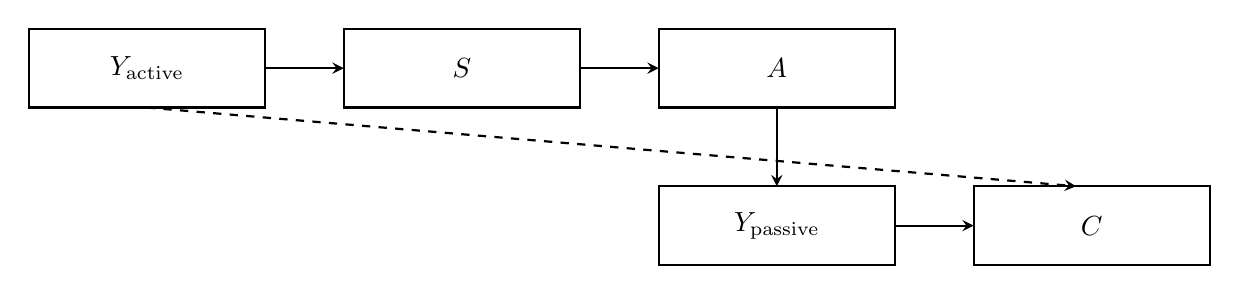
\begin{tikzpicture}[>=stealth, thick]
\draw (0,0) rectangle (3,1);
\node at (1.5,0.5) {$Y_{\mathrm{active}}$};

\draw (4,0) rectangle (7,1);
\node at (5.5,0.5) {$S$};

\draw (8,0) rectangle (11,1);
\node at (9.5,0.5) {$A$};

\draw (8,-2) rectangle (11,-1);
\node at (9.5,-1.5) {$Y_{\mathrm{passive}}$};

\draw (12,-2) rectangle (15,-1);
\node at (13.5,-1.5) {$C$};

\draw[->] (3,0.5)--(4,0.5);
\draw[->] (7,0.5)--(8,0.5);
\draw[->] (9.5,0)--(9.5,-1);
\draw[->] (11,-1.5)--(12,-1.5);

\draw[->, dashed] (1.5,0)--(13.3,-1);
\end{tikzpicture}
\end{figure}

The solid path is the lecture's recommended sequence: earned income becomes surplus, surplus thickens the asset base, the asset base throws off passive cash flow, and only then does consumption become easy. The dashed line is the path Eric criticizes: active income runs straight to lifestyle and leaves no river behind.

\section{Ryan: Revenue, Valuation, Belief, and Compounding}

After the Eric segment, the lecture does something important. It recaps his lesson and then reopens the inquiry through another speaker. This prevents the chapter from becoming a single case study. Ryan shifts the topic from pure asset cash flow toward enterprise value, belief, compounding, and sales.

Ryan says he has been an entrepreneur for roughly a decade, has started and scaled multiple businesses, and now manages roughly \(800\) e-commerce stores on Amazon. The first numerical point is not just his annual performance but the distinction between revenue and value:
\begin{align}
R_{\text{Ryan}} &\approx \$35\,\text{M},\\
V_{\text{Ryan}} &\approx \$140\,\text{M}.
\end{align}
He insists that these are not the same object. The lecture thus widens its concept of wealth:
\begin{equation}
V \neq \text{current monthly cash flow}.
\end{equation}

This matters because Ryan's explicit argument is temporal. Many people, he says, optimize for current cash extraction and therefore fail to build sale value. But if one knew that a business could be sold for \$100 million or \$200 million in several years, one might rationally accept lower near-term personal cash. In other words, the lecture distinguishes between money that arrives now and value that is being built.

Ryan then inserts a second layer, not exactly mathematical but causal: belief systems. He says that what one treats as normal or possible alters what one will attempt, what one will tolerate, and therefore what one can build. We should not turn this into pseudo-science. But within the lecture it plays a specific role. It explains why the same external world generates different entrepreneurial trajectories.

The most delicate part of Ryan's segment concerns compounding through overfunded whole life or IUL-type structures. Here caution is essential. We record the mechanism as his claim, not as settled doctrine. His description is that one places money into the policy, lets it compound, and simultaneously borrows against it:
\begin{align}
L &= \lambda P,\qquad 0.8 \le \lambda \le 0.9,\\
P_{t+1} &= P_t(1+r).
\end{align}
Here \(P\) denotes the policy value, \(L\) the collateralized loan, and \(\lambda\) the loan-to-value fraction he quotes.

The intended logic is straightforward. If money is spent directly on consumption, it is used once. If it remains parked in a compounding structure while one borrows against it, then in Ryan's telling it is doing two jobs at once: it continues compounding while also financing present use. The lecture does not prove this in full institutional detail, and we should not pretend that it does. But the narrative function is clear. Ryan adds a model of capital reuse to Eric's earlier stock-and-flow model.

He closes by returning to a simpler law: without sales there is no money. We may write that as
\begin{equation}
\text{Sales} = \text{value offered} \mapsto \text{money received}.
\end{equation}
This is less a formula than a sharpening of the lecture's attitude. Money does not appear by magic. It appears when someone pays for perceived value.

\section{James: Attention as a Revenue Engine}

James narrows the field and makes a different claim. He works in watches, jewelry, and cars, and he says his operation generates more than nine figures in revenue each year. His strongest conceptual contribution is the insistence that social media and marketing are not cosmetic. They are productive assets.

The lecture's qualitative funnel may be written as
\begin{equation}
\text{attention} \longrightarrow \text{trust} \longrightarrow \text{sales} \longrightarrow R.
\end{equation}
James states the point provocatively. He says he would rather have a billion followers than a billion dollars, and he adds that with roughly \(250{,}000\) followers he is already driving nine digits of revenue:
\begin{equation}
F \approx 250{,}000 \;\Longrightarrow\; R \text{ in nine figures},
\end{equation}
where the implication is understood as his own commercial experience, not as a universal conversion law.

What matters is the lecture's broader theme. Once again the visible luxury object is not primary. Audience is a vehicle. Distribution is a vehicle. Marketing reach is a vehicle. The interview thus extends the list of wealth-generating structures beyond real estate and operating business equity.

James's financial advice is interesting precisely because it is not the same as Eric's. He says one should not obsess over every small expense, but should instead focus on making more and enabling throughput. That is not a contradiction of Eric so much as a different emphasis. Eric warns against burning high active income on lifestyle; James warns against small-minded cost fixation when scale and sales are the true bottlenecks. The chapter should preserve both voices without collapsing them into a single rule.

\section{Justin Waller: Scaling by Staying, Selling by Conviction}

The last major movement of the lecture returns to construction and real estate, now with a different emphasis. Justin Waller says he has been at it for about fifteen years; he gives current business scale on the order of \$30 million in revenue and about \$5 million in personal income. But the conceptual burden of his section is not the number. It is what persistence does to judgment.

His first principle is concentration. People, he says, bounce from one business to another as soon as they are hit hard. But the operator who stays in one business long enough begins to recognize the blows before they land. This is a learning curve, and the lecture presents it as the real mechanism of scaling.

In words, the model is
\begin{equation}
\text{repetition in one line of business} \longrightarrow \text{pattern recognition} \longrightarrow \text{scale}.
\end{equation}
His image is memorable: one waters one tree until it bears fruit.

The second principle is sales with conviction. In construction, he says, the lower bid is not always the better economic choice, because delays are costly. We may formalize the buyer's problem in the simple inequality
\begin{equation}
\Delta P < \text{Cost of schedule delay}.
\end{equation}
Here \(\Delta P\) is the premium charged by the more reliable contractor. If the expected loss from delay is larger than that premium, then paying more is rational. Justin's point is that the seller who truly believes he can hit schedule can sell above the cheapest number because he is reducing a different, often larger, cost for the client.

This is a beautiful moment in the lecture because it translates conviction into economics. Conviction is not just swagger. It is a claim about the buyer's optimization problem.

Justin then widens the frame again. Physical discipline, fitness, sobriety in youth, and the refusal to dissolve oneself into bad company are all presented as economic conditions. The lecture is not saying that biceps generate revenue by themselves. It is saying that discipline is legible. It changes how others price one's promises. It changes whether one's word is taken seriously. That is still part of the machinery.

\section{Closing Synthesis: Vehicles, Not Trophies}

We can now state the lecture's governing pattern in one line. Wealth is not described here as a static number but as a sequence:
\begin{align}
\text{business effort} &\longrightarrow \text{income},\\
\text{income} &\longrightarrow \text{assets, equity, or audience},\\
\text{assets, equity, or audience} &\longrightarrow \text{cash flow or valuation},\\
\text{cash flow or valuation} &\longrightarrow \text{luxury only at the end}.
\end{align}

That is why the lecture keeps returning to the word \emph{vehicle}. A business is a vehicle. Real estate is a vehicle. Audience is a vehicle. Valuation is a vehicle. Even discipline, in the stronger parts of the lecture, is treated as a vehicle because it enables the others to function.

The chapter should therefore leave the reader with a very sharp distinction. A car is not the theorem. A car is the corollary. The theorem is that if active income is consumed immediately, wealth thins out into a pile; if surplus is converted into structures that keep paying, wealth begins to behave like a river. The various interviewees disagree about tactics, emphasis, and temperament, but on that much the lecture is remarkably consistent.